\PassOptionsToPackage{unicode=true}{hyperref} % options for packages loaded elsewhere
\PassOptionsToPackage{hyphens}{url}
%
\documentclass[]{book}
\usepackage{lmodern}
\usepackage{amssymb,amsmath}
\usepackage{ifxetex,ifluatex}
\usepackage{fixltx2e} % provides \textsubscript
\ifnum 0\ifxetex 1\fi\ifluatex 1\fi=0 % if pdftex
  \usepackage[T1]{fontenc}
  \usepackage[utf8]{inputenc}
  \usepackage{textcomp} % provides euro and other symbols
\else % if luatex or xelatex
  \usepackage{unicode-math}
  \defaultfontfeatures{Ligatures=TeX,Scale=MatchLowercase}
\fi
% use upquote if available, for straight quotes in verbatim environments
\IfFileExists{upquote.sty}{\usepackage{upquote}}{}
% use microtype if available
\IfFileExists{microtype.sty}{%
\usepackage[]{microtype}
\UseMicrotypeSet[protrusion]{basicmath} % disable protrusion for tt fonts
}{}
\IfFileExists{parskip.sty}{%
\usepackage{parskip}
}{% else
\setlength{\parindent}{0pt}
\setlength{\parskip}{6pt plus 2pt minus 1pt}
}
\usepackage{hyperref}
\hypersetup{
            pdftitle={Reproducible Medical Research with R},
            pdfauthor={Peter D.R. Higgins, MD, PhD, MSc},
            pdfborder={0 0 0},
            breaklinks=true}
\urlstyle{same}  % don't use monospace font for urls
\usepackage{color}
\usepackage{fancyvrb}
\newcommand{\VerbBar}{|}
\newcommand{\VERB}{\Verb[commandchars=\\\{\}]}
\DefineVerbatimEnvironment{Highlighting}{Verbatim}{commandchars=\\\{\}}
% Add ',fontsize=\small' for more characters per line
\usepackage{framed}
\definecolor{shadecolor}{RGB}{248,248,248}
\newenvironment{Shaded}{\begin{snugshade}}{\end{snugshade}}
\newcommand{\AlertTok}[1]{\textcolor[rgb]{0.94,0.16,0.16}{#1}}
\newcommand{\AnnotationTok}[1]{\textcolor[rgb]{0.56,0.35,0.01}{\textbf{\textit{#1}}}}
\newcommand{\AttributeTok}[1]{\textcolor[rgb]{0.77,0.63,0.00}{#1}}
\newcommand{\BaseNTok}[1]{\textcolor[rgb]{0.00,0.00,0.81}{#1}}
\newcommand{\BuiltInTok}[1]{#1}
\newcommand{\CharTok}[1]{\textcolor[rgb]{0.31,0.60,0.02}{#1}}
\newcommand{\CommentTok}[1]{\textcolor[rgb]{0.56,0.35,0.01}{\textit{#1}}}
\newcommand{\CommentVarTok}[1]{\textcolor[rgb]{0.56,0.35,0.01}{\textbf{\textit{#1}}}}
\newcommand{\ConstantTok}[1]{\textcolor[rgb]{0.00,0.00,0.00}{#1}}
\newcommand{\ControlFlowTok}[1]{\textcolor[rgb]{0.13,0.29,0.53}{\textbf{#1}}}
\newcommand{\DataTypeTok}[1]{\textcolor[rgb]{0.13,0.29,0.53}{#1}}
\newcommand{\DecValTok}[1]{\textcolor[rgb]{0.00,0.00,0.81}{#1}}
\newcommand{\DocumentationTok}[1]{\textcolor[rgb]{0.56,0.35,0.01}{\textbf{\textit{#1}}}}
\newcommand{\ErrorTok}[1]{\textcolor[rgb]{0.64,0.00,0.00}{\textbf{#1}}}
\newcommand{\ExtensionTok}[1]{#1}
\newcommand{\FloatTok}[1]{\textcolor[rgb]{0.00,0.00,0.81}{#1}}
\newcommand{\FunctionTok}[1]{\textcolor[rgb]{0.00,0.00,0.00}{#1}}
\newcommand{\ImportTok}[1]{#1}
\newcommand{\InformationTok}[1]{\textcolor[rgb]{0.56,0.35,0.01}{\textbf{\textit{#1}}}}
\newcommand{\KeywordTok}[1]{\textcolor[rgb]{0.13,0.29,0.53}{\textbf{#1}}}
\newcommand{\NormalTok}[1]{#1}
\newcommand{\OperatorTok}[1]{\textcolor[rgb]{0.81,0.36,0.00}{\textbf{#1}}}
\newcommand{\OtherTok}[1]{\textcolor[rgb]{0.56,0.35,0.01}{#1}}
\newcommand{\PreprocessorTok}[1]{\textcolor[rgb]{0.56,0.35,0.01}{\textit{#1}}}
\newcommand{\RegionMarkerTok}[1]{#1}
\newcommand{\SpecialCharTok}[1]{\textcolor[rgb]{0.00,0.00,0.00}{#1}}
\newcommand{\SpecialStringTok}[1]{\textcolor[rgb]{0.31,0.60,0.02}{#1}}
\newcommand{\StringTok}[1]{\textcolor[rgb]{0.31,0.60,0.02}{#1}}
\newcommand{\VariableTok}[1]{\textcolor[rgb]{0.00,0.00,0.00}{#1}}
\newcommand{\VerbatimStringTok}[1]{\textcolor[rgb]{0.31,0.60,0.02}{#1}}
\newcommand{\WarningTok}[1]{\textcolor[rgb]{0.56,0.35,0.01}{\textbf{\textit{#1}}}}
\usepackage{longtable,booktabs}
% Fix footnotes in tables (requires footnote package)
\IfFileExists{footnote.sty}{\usepackage{footnote}\makesavenoteenv{longtable}}{}
\usepackage{graphicx,grffile}
\makeatletter
\def\maxwidth{\ifdim\Gin@nat@width>\linewidth\linewidth\else\Gin@nat@width\fi}
\def\maxheight{\ifdim\Gin@nat@height>\textheight\textheight\else\Gin@nat@height\fi}
\makeatother
% Scale images if necessary, so that they will not overflow the page
% margins by default, and it is still possible to overwrite the defaults
% using explicit options in \includegraphics[width, height, ...]{}
\setkeys{Gin}{width=\maxwidth,height=\maxheight,keepaspectratio}
\setlength{\emergencystretch}{3em}  % prevent overfull lines
\providecommand{\tightlist}{%
  \setlength{\itemsep}{0pt}\setlength{\parskip}{0pt}}
\setcounter{secnumdepth}{5}
% Redefines (sub)paragraphs to behave more like sections
\ifx\paragraph\undefined\else
\let\oldparagraph\paragraph
\renewcommand{\paragraph}[1]{\oldparagraph{#1}\mbox{}}
\fi
\ifx\subparagraph\undefined\else
\let\oldsubparagraph\subparagraph
\renewcommand{\subparagraph}[1]{\oldsubparagraph{#1}\mbox{}}
\fi

% set default figure placement to htbp
\makeatletter
\def\fps@figure{htbp}
\makeatother

\usepackage{booktabs}
\usepackage{amsthm}
\makeatletter
\def\thm@space@setup{%
  \thm@preskip=8pt plus 2pt minus 4pt
  \thm@postskip=\thm@preskip
}
\makeatother
\usepackage[]{natbib}
\bibliographystyle{apalike}

\title{Reproducible Medical Research with R}
\author{Peter D.R. Higgins, MD, PhD, MSc}
\date{2020-04-04}

\begin{document}
\maketitle

{
\setcounter{tocdepth}{1}
\tableofcontents
}
\hypertarget{preface}{%
\chapter{Preface}\label{preface}}

Welcome to Reproducible Medical Research with R (RMWR). I hope that this book meets your needs.

\hypertarget{who-this-book-is-for}{%
\section{Who This Book is For}\label{who-this-book-is-for}}

This is a book for anyone in the medical field interested in analyzing the data available to them to better understand health, disease, or delivery of care. This could include nurses, dieticians, psychologists, and PhDs in related fields, as well as medical students, residents, fellows, or doctors in practice.\\
I expect that most learners will be using this book in their spare time at night and on weekends, as the medical school curriculum is already packed full, and there is no room to add skills in reproducible research to the standard curriculum. This book is designed for self-teaching, and many hints and solutions will be provided to avoid roadblocks and frustration.
Many learners find themselves wanting to develop reproducible research skills after they have finished their training, and after they have become comfortable with their clinical role. This is the time when they identify and want to address problems in their practice with the data they have before them. This book is for you.

\hypertarget{the-spiral-of-success-structure}{%
\section{The Spiral of Success Structure}\label{the-spiral-of-success-structure}}

This book is structured on the concept of a ``spiral of success'', with readers learning about topics like data visualization, data wrangling, data modeling, reproducible research, and communication of results in repeated passes. These will initially be at a superficial level, and at each pass of the spiral, will provide increasing depth and complexity. This means that the chapters on data wrangling will not all be together, nor the chapters on data visualization. Our goal is to build skills gradually, and return to (and remind students of) their previously built skills in one area and to add to them. The eventual goal is for learners to be able to produce, document, and communicate reproducible research to their community.

\hypertarget{motivation-for-this-book}{%
\section{Motivation for this Book}\label{motivation-for-this-book}}

Most medical people who learn R to do their own data analysis do it on their own time. They rarely have time for a semester-long course, and their clinical schedules usually will not allow it. Fortunately, a lot of people learn R on their own, and there is a strong and supportive R Community to help new learners. A 2019 Twitter survey conducted by \texttt{@RLadies} found that more than half of respondents were largely self-taught, from books and online resources.

There are a lot of good resources for learning R, so why one more? In part, because the needs of a medical audience are often different. There are distinct needs for protecting health information, generating a descriptive Table One, using secure data tools like REDCap, and creating standard medical journal and meeting output in Word, Powerpoint, and poster formats.

More and more, all science is becoming data science. We are able to track patients, their test results, and even the individual pixels (voxels) of their CT scans electronically, and use those data points to develop new knowledge. While one could argue that health care workers should collect data and bring it to trained statisticians, this does not work nearly as well as you might expect. Most academic statisticians are incentivized to develop new statistical methods, and are not very interested (or incentivized) to do the hand-holding required to wrangle messy clinical data into a manuscript.

There also are simply not enough statisticians to meet the needs of medical science. Having clinicians on the front lines with some data science training makes a big difference, whether in 1854 in London (John Snow) or in 2014 in Flint, Michigan (Mona Hanna-Atisha). Having more clinicians with some training will impact medical care, as they will identify local problems that would have otherwise never reached a statistician, and probably never been addressed with data otherwise.

\hypertarget{the-scientific-reproducibility-crisis}{%
\section{The Scientific Reproducibility Crisis}\label{the-scientific-reproducibility-crisis}}

Beginning as far back as 1989, with the David Baltimore case, and increasingly publicly through the 2010s, there has been a rising tide of realization that a lot of taxpayer-funded science is done sloppily, and that our standards as scientists need to be higher. The line between carelessly-done science and outright fraud is a thin one, and the case can be made that doing science in a sloppy fashion defrauds the funders, as it leads to results that can not be reproduced nor replicated. Particularly in medicine, where incorrect findings can cause great harm, we should take special care to do scientific research which is well-documented, reproducible, and replicable. This topic as a motivating force for doing careful medical research will be expanded upon in Chapter 1.

\hypertarget{what-this-book-is-not}{%
\section{What this Book is Not}\label{what-this-book-is-not}}

\hypertarget{this-book-is-not-a-statistics-text}{%
\subsection{This Book is Not A Statistics Text}\label{this-book-is-not-a-statistics-text}}

This is not an introduction to statistics. I am assuming that you have learned some statistics somewhere in secondary school, undergraduate studies, graduate school, or even medical school. There are lots of statisticians with Ph.D.s who can certainly teach statistics much more effectively than I can. While I have a master's degree in Clinical Research Design and Statistical Analysis (isn't that a mouthful!) from the University of Michigan, I will leave formal teaching of statistics to the pros.

If you need to brush up on your statistics, no worries. There are several excellent (and free!) e-books on that very topic, using R. Some good examples include (go ahead and click through the blue links to explore):

\begin{enumerate}
\def\labelenumi{\arabic{enumi}.}
\tightlist
\item
  \href{https://learningstatisticswithr-bookdown.netlify.com}{Learning Statistics with R (LSR)}
\item
  \href{https://bookdown.org/fjmcgrade/ismaykim/}{Modern Dive}
\item
  \href{https://tinystats.github.io/teacups-giraffes-and-statistics/index.html}{Teacup Giraffes}
\end{enumerate}

We will cover a lot of the same materials as these books, but with a less theoretical and more applied approach. I will focus on specific medical examples, and emphasize issues (like Protected Health Information) that are particularly important for medical data. I am assuming that you are here because you want to analyze your own data in your probably very limited free time.

\hypertarget{this-book-does-not-provide-comprehensive-coverage-of-the-r-universe}{%
\subsection{This Book Does Not Provide Comprehensive Coverage of the R Universe}\label{this-book-does-not-provide-comprehensive-coverage-of-the-r-universe}}

This book is also far from comprehensive in teaching what is available in the R ecosystem. This book should be considered a launch pad. Many of the later chapters will give you a taste of what is available in certain areas, and guide you to resources (and links) that you can explore to learn more and do more beyond the scope of this book.

\hypertarget{intro}{%
\chapter{Getting Started and Installing}\label{intro}}

To do medical data science in R, you first need up-to-date tools. In this chapter, we will get you started by installing R and then RStudio on your computer to get you started with R. Then we will help you install git on your computer as a first step into version control. We will walk you through the RStudio coding environment to get you ready for data visualization and producing a data communication product to share with friends and colleagues.

You can label chapter and section titles using \texttt{\{\#label\}} after them, e.g., we can reference Chapter \ref{intro}. If you do not manually label them, there will be automatic labels anyway, e.g., Chapter \ref{methods}.

Figures and tables with captions will be placed in \texttt{figure} and \texttt{table} environments, respectively.

\begin{Shaded}
\begin{Highlighting}[]
\KeywordTok{par}\NormalTok{(}\DataTypeTok{mar =} \KeywordTok{c}\NormalTok{(}\DecValTok{4}\NormalTok{, }\DecValTok{4}\NormalTok{, }\FloatTok{.1}\NormalTok{, }\FloatTok{.1}\NormalTok{))}
\KeywordTok{plot}\NormalTok{(pressure, }\DataTypeTok{type =} \StringTok{'b'}\NormalTok{, }\DataTypeTok{pch =} \DecValTok{19}\NormalTok{)}
\end{Highlighting}
\end{Shaded}

\begin{figure}

{\centering 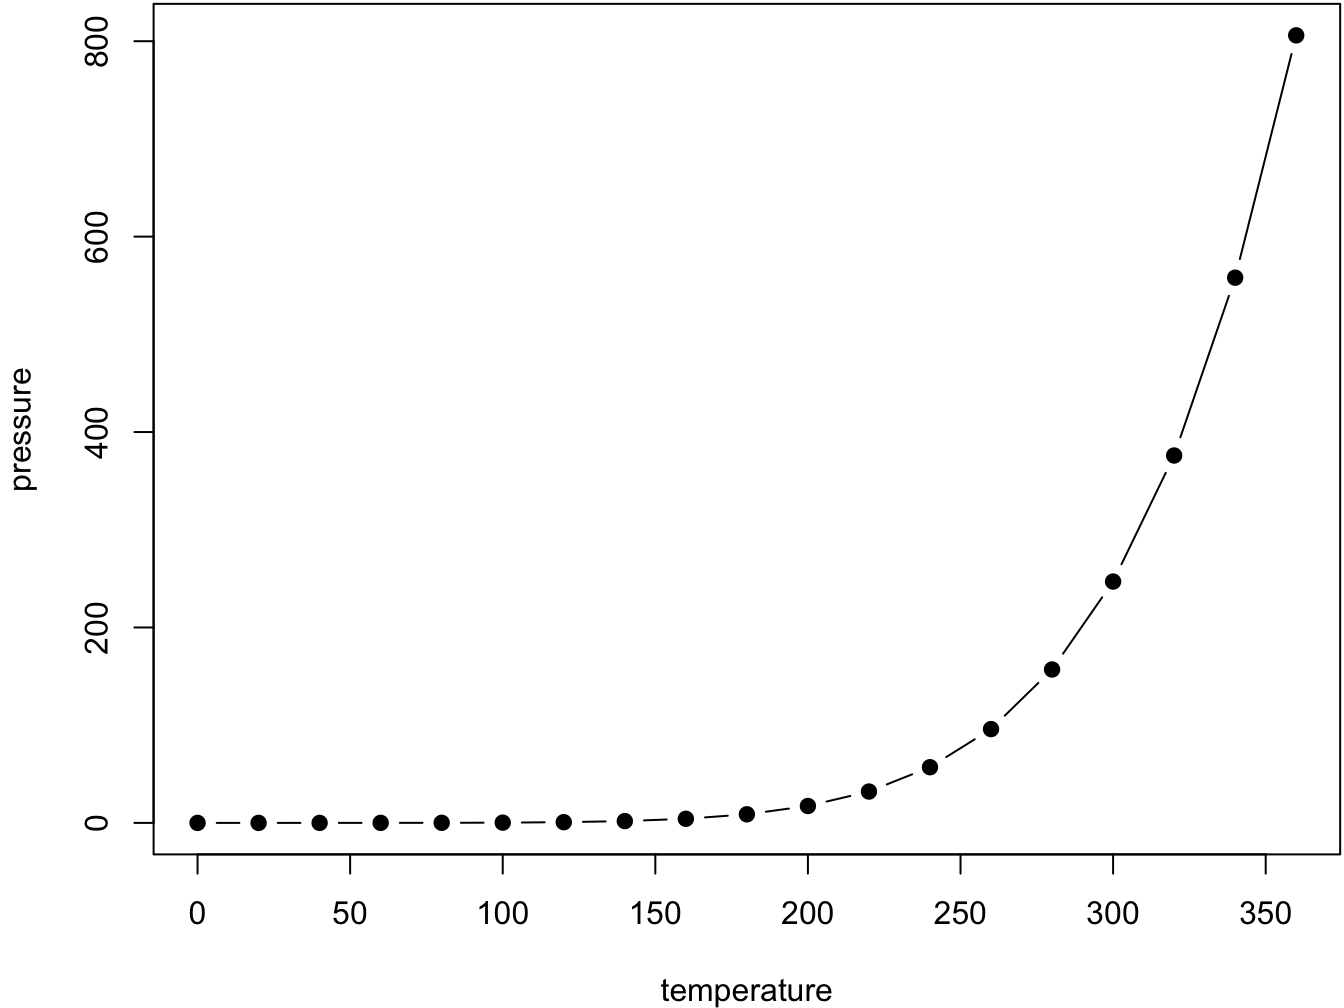
\includegraphics[width=0.8\linewidth]{rmrwr_files/figure-latex/nice-fig-1} 

}

\caption{Here is a nice figure!}\label{fig:nice-fig}
\end{figure}

Reference a figure by its code chunk label with the \texttt{fig:} prefix, e.g., see Figure \ref{fig:nice-fig}. Similarly, you can reference tables generated from \texttt{knitr::kable()}, e.g., see Table \ref{tab:nice-tab}.

\begin{Shaded}
\begin{Highlighting}[]
\NormalTok{knitr}\OperatorTok{::}\KeywordTok{kable}\NormalTok{(}
  \KeywordTok{head}\NormalTok{(iris, }\DecValTok{20}\NormalTok{), }\DataTypeTok{caption =} \StringTok{'Here is a nice table!'}\NormalTok{,}
  \DataTypeTok{booktabs =} \OtherTok{TRUE}
\NormalTok{)}
\end{Highlighting}
\end{Shaded}

\begin{table}

\caption{\label{tab:nice-tab}Here is a nice table!}
\centering
\begin{tabular}[t]{rrrrl}
\toprule
Sepal.Length & Sepal.Width & Petal.Length & Petal.Width & Species\\
\midrule
5.1 & 3.5 & 1.4 & 0.2 & setosa\\
4.9 & 3.0 & 1.4 & 0.2 & setosa\\
4.7 & 3.2 & 1.3 & 0.2 & setosa\\
4.6 & 3.1 & 1.5 & 0.2 & setosa\\
5.0 & 3.6 & 1.4 & 0.2 & setosa\\
\addlinespace
5.4 & 3.9 & 1.7 & 0.4 & setosa\\
4.6 & 3.4 & 1.4 & 0.3 & setosa\\
5.0 & 3.4 & 1.5 & 0.2 & setosa\\
4.4 & 2.9 & 1.4 & 0.2 & setosa\\
4.9 & 3.1 & 1.5 & 0.1 & setosa\\
\addlinespace
5.4 & 3.7 & 1.5 & 0.2 & setosa\\
4.8 & 3.4 & 1.6 & 0.2 & setosa\\
4.8 & 3.0 & 1.4 & 0.1 & setosa\\
4.3 & 3.0 & 1.1 & 0.1 & setosa\\
5.8 & 4.0 & 1.2 & 0.2 & setosa\\
\addlinespace
5.7 & 4.4 & 1.5 & 0.4 & setosa\\
5.4 & 3.9 & 1.3 & 0.4 & setosa\\
5.1 & 3.5 & 1.4 & 0.3 & setosa\\
5.7 & 3.8 & 1.7 & 0.3 & setosa\\
5.1 & 3.8 & 1.5 & 0.3 & setosa\\
\bottomrule
\end{tabular}
\end{table}

You can write citations, too. For example, we are using the \textbf{bookdown} package \citep{R-bookdown} in this sample book, which was built on top of R Markdown and \textbf{knitr} \citep{xie2015}.

\hypertarget{literature}{%
\chapter{Literature}\label{literature}}

Here is a review of existing methods.

\hypertarget{methods}{%
\chapter{Methods}\label{methods}}

We describe our methods in this chapter.

\hypertarget{applications}{%
\chapter{Applications}\label{applications}}

Some \emph{significant} applications are demonstrated in this chapter.

\hypertarget{example-one}{%
\section{Example one}\label{example-one}}

\hypertarget{example-two}{%
\section{Example two}\label{example-two}}

\hypertarget{final-words}{%
\chapter{Final Words}\label{final-words}}

We have finished a nice book.

\bibliography{book.bib,packages.bib}

\end{document}
